\documentclass{iopconfser}
\usepackage{float}
\usepackage{graphicx}
\usepackage{subcaption}
\usepackage[automake]{glossaries-extra}
\usepackage{ragged2e}
\usepackage[export]{adjustbox}
\usepackage{mathtools}
\usepackage{setspace}
\usepackage{dirtytalk}

\onehalfspacing
% \makeglossaries

\setabbreviationstyle[acronym]{long-postshort-user}
\glssetcategoryattribute{acronym}{nohyperfirst}{true}
\setabbreviationstyle{short-nolong}
\makeglossaries

% --------------------
% ---- Glossaries ----
% --------------------
\newglossaryentry{asyncio}{name=Asyncio, description={A Python library for asynchronous code.}}
\newglossaryentry{stim}{name=STIM300, description={A MEMS-based \gls{imu}}}
\newglossaryentry{f9p}{name=F9P, description={A Global Navigation Satellite System (GNSS) receiver manufactured by u-blox.}}

% --------------------
% ----- Acronyms -----
% --------------------
\newacronym{asv}{ASV}{Autonomous Surface Vehicle}
\newacronym{dolp}{DoLP}{Degree of Linear Polarization}
\newacronym{aolp}{AoLP}{Angle of Linear Polarization}
\newacronym{sitaw}{SITAW}{Situational Awareness}
\newacronym{poe}{PoE}{Power over Ethernet}
\newacronym{pps}{PPS}{Pulse Per Second}
\newacronym{cpfa}{CPFA}{Color-Polarization Filter Array}
\newacronym{utc}{UTC}{Coordinated Universal Time}
\newacronym{imu}{IMU}{Inertial Measurement Unit}
\newacronym{tov}{TOV}{Time of Validity}
\newacronym{tm2}{TM2}{Time mark data}
\newacronym{gnss}{GNSS}{Global Navigation Satellite System}
\newacronym{ptp}{PTP}{Precision Time Protocol}

% \glsaddall
% \makenoidxglossaries

% \glsunset{cpu}
\glsunset{gnss}
\glsunset{imu}
\glsunset{tm2}
\glsunset{utc}

% --------------------
% ----- Shortcuts ----
% --------------------


\addbibresource{mylib.bib}


\begin{document}
\title{IØ8906 Submission}
% \author{Emil Martens}

\section*{Utilization Plan}
\subsection*{Problem / Solution}
I started my pitch by asking the audience to raise a hand if they depend on data to perform their research.
With 100\% of the audience raising their hand, it is clear that data is a crucial part of research.
Of course, the type of data each researcher needs varies, but in the field of robotics and autonomy, almost every researcher needs to work with some sort of sensor data.
With this in mind, I have developed a sensor rig, depicted in Figure \ref{fig:operation}, to make it easier for researchers to perform data collection.

The sensor rig is designed for easy transport and operation by a single individual. 
It can also be temporarily attached to an existing vessel, making it versatile for various data collection scenarios.
Accurate positioning and synchronization are essential for any high-quality dataset, so the sensor rig is equipped with two GNSS receivers and an IMU for accurate positioning.
Additionally, the main computer and all the sensors have been accurately synchronized to UTC.
The sensor rig provides four separate gigabit ethernet ports with PoE to connect various sensors.
A custom web app has been developed to control and monitor the sensor rig from a smartphone, making it easy for almost anyone to operate it.
Multiple people have used the sensor signature with minimal training, a testament to its usability.

At the end of the pitch I asked for funding hire a student over the summer to help developing the sensor rig further and use it collect data.
From holding a similar pitches in the past did get funding to hire not one but two students, signalling that the audience sees the potential in the sensor rig.

From the pitching panel I goot good feedback on the pitch, but they pointed out that my ask could be formulated more clarly.


\begin{figure}[H]
    \centering
    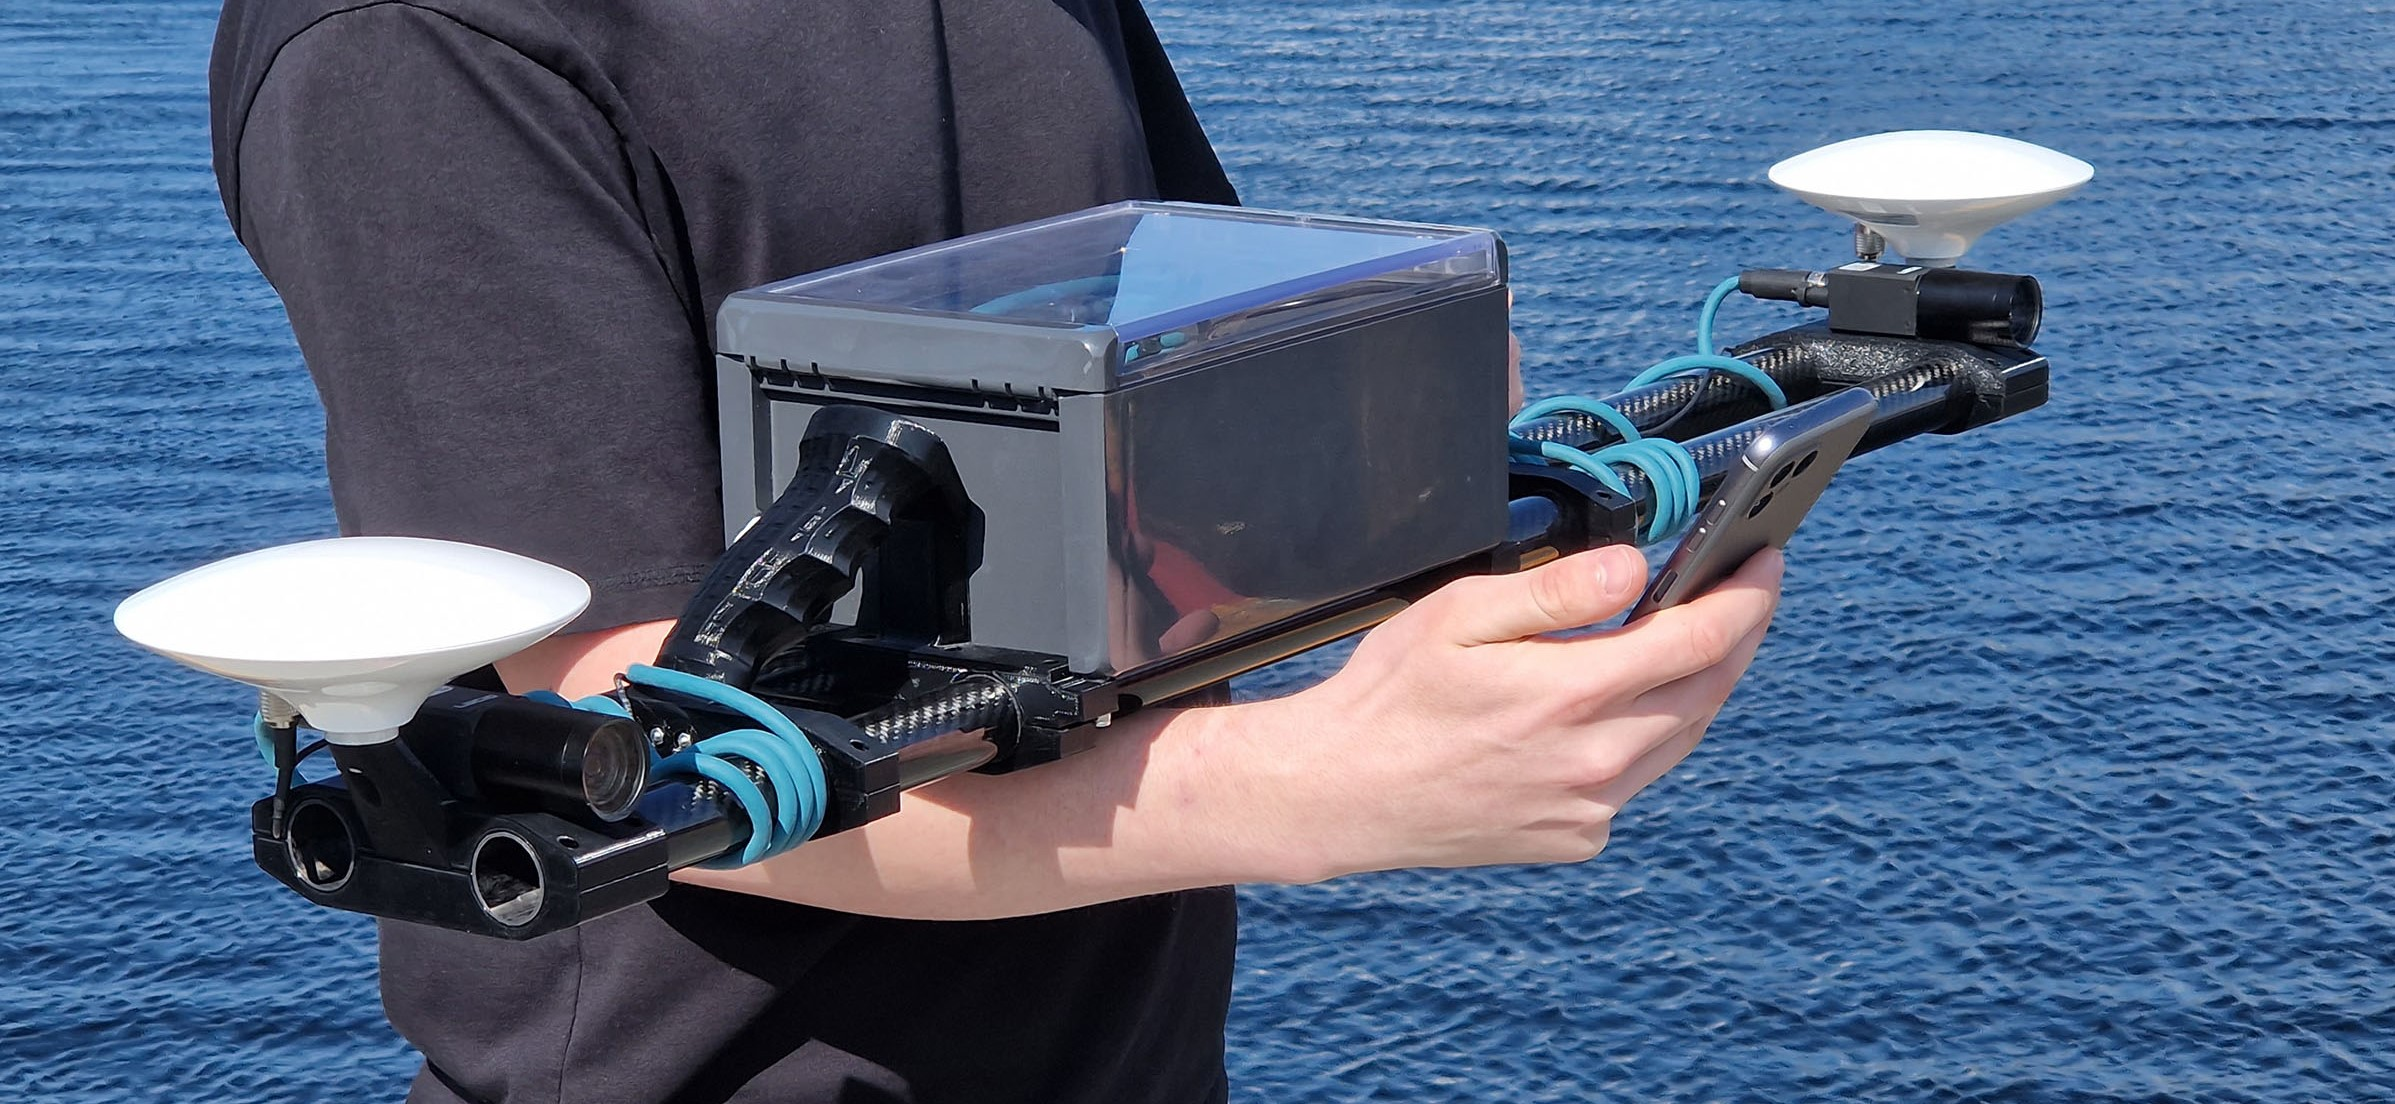
\includegraphics[trim={0 1cm 0 1cm},clip,width=\textwidth]{figures/operation.jpg}
    \caption{Human operation of the sensor rig with monitoring over a smartphone. \label{fig:operation}}
\end{figure}


\subsection*{Benefits}
From a user's perspective, the key benefit of the sensor rig is its ease of use.
Research teams working with autonomy often rely on expensive research vehicles, such as the autonomous ferry Milliampere 2, to do their research.
These vehicles can be used to collect data, but it can be overkill, and their operation often requires planning and coordination between multiple people.
If anything fails on the vehicle, even things not connected to data collection, such as a motor, the vehicle is generally taken out of operation.

With the sensor rig, a single person can just pick it up, walk outside and start collecting data in a matter of minutes.
With its modular and stand alone desagn, it is also easy to attach it to an existing vehicle to temporarily create a pseudo research vehicle or expand the capabilities of an existing one.
Compared to any research vehicle, the sensor rig is also much cheaper, making it more accessible to smaller research teams.

\subsection*{Market potential}
If the sensor rig was to be commercialized, it would be targeted towards small to medium sized research teams working in autonomy, as larger teams probably have dedicated hardware engineers to develop custom solutions.
A potential product would be a barebones sensor rig equipped only with GNSS receivers, an IMU, and a core computer.
Different brackets for attaching various sensors could be sold separately, as well as fully equipped versions with cameras and other sensors.
As the sensors used for researching autonomy are generally expensive, it is valuable to have an easy way to use them as much as possible.
From personal experience, I know researchers often have expensive sensors lying around that they do not use because they are not usable.

The market potential for the sensor rig remains to be researched, but based on feedback from other researchers, I believe there is a market for a product like this.

\subsection*{User vs Customer}
As was discussed in the course, the user and the customer are not always the same person.
In the case of the sensor rig, the user is the researcher who uses the sensor rig to collect data, while the customer is the research institution or the research team that buys the sensor rig.
Hovewer I think it is far to assume researchers generally have a say in what equipment they use, so the user and the customer are likely to be the same person in practice.

\subsection*{Existing competition}
I have not yet done a market analysis, but I am unaware of any similar product on the market.
One related product is the ZED-box from Stereolabs, which can be used to collect data from multiple ZED cameras and synchronize them to UTC \cite{stereolabsZEDBoxEmbedded}. 
This is not a competitor to the sensor rig, but shows that there is a market for easy to use sensor synchronization systems.
Another related product is the SentiBoard from SentiSystems, which handles the synchronization of multiple sensors and can be used to calculate accurate position and orientation from GNSS and IMU data \cite{sentisystemsSentiSystemsSolutions}.
Both the ZED box and the SentiBoard appear to be more aimed at the industrial market and are not as versatile as the sensor rig.

\subsection*{Milestones}
The first milestone for the sensor rig was to develop a prototype and test it in a natural research setting.
This milestone was reached in 2024, and the sensor rig has since been in use to collect data.
I submitted a paper describing the sensor rig to the ICMASS 2024 conference, which was accepted, and I will present it there.
This is the next milestone, and it will be an excellent opportunity to get feedback from the research community and to get the sensor rig known.

My goal is to use the data from the sensor rig in my future publications and have other researchers use it in their research as well, proving the sensor rig's value in a research setting.
Hopefully, when I finish my PhD in two years, the sensor rig will have a proven track record and be ready for commercialization.

If I decide to pursue commercialization, the following milestone would be to sell a couple of units to other research teams and provide good customer support to get feedback on the product.
Doing this should require little investment, as the buyer will cover the bill of materials. It can be done as a side job if I reduce my main job to part-time.

The end goal would be to sell the sensor rig as a finished product with a thorough user guide and have it used by research teams worldwide with minimal support.


\subsection*{Possible Challenges}
I think the main challene with the product is that it might be that researchers often have very specific needs for their data collection, and the sensor rig might be to general to hit any specific need.
Striking the right balance between modularity and ease of use will be crucial for the sensor rig's success.
The primary way to solve this is to have many different people use it during my PhD and get feedback on how the rig adapts to their needs.

\subsection*{Commencialization}
A key advantage of commercializing the sensor rig is that it requires little investment to get started. 
The rig is an assembly of off-the-shelf components and 3D-printed parts coupled with software already developed.
Initially, it would be possible to order all the components after a sale and assemble the sensor rig in a few days.
It will imply some lead time, but it should not be significantly longer than the lead time of the components themselves.

In the beginning, it would make most sense to order the 3D-printed parts from a 3D printing service, but if the demand is high enough, it would make sense to invest in an industrial SLS 3D printer to make the parts in-house.
If the demand for the sensors and hardware used in the sensor rig is high enough, becoming a certified reseller of the sensors and electronic components would also make sense to increase the margins.

\subsection*{Intelectual Property}
I do not consider intellectual property a big concern for the sensor rig.
The value in buying it would be in the ease of use and the fact that it is a complete solution that does not require any development.
People willing to invest the time and effort to reverse engineer the sensor rig could make something similar anyways.

However, if I were to pursue commercialization, I would seek advice from Hans-Christian Bloom or others at the TTO to see if any parts of the sensor rig are worth patenting.
Also, as he mentioned in his lecture, the value of a patent is not only in the patent itself but in the fact that it makes it easier to get funding and to sell the product \cite{blomIntelectualProperty2024}.

\pagebreak
\section*{Reflection Note on My Role}

\subsection*{Developer}
A natural role for me in the commercialization process would be as the main developer, and I would continue to develop the sensor rig.
Being the developer and main user of the sensor rig, I have a unique understanding of both the product and the needs I face as a researcher in the field, which would be hard to replace.
At the beginning of the design process, I designed the sensor rig primarily to fit my own needs but with a strong focus on making it easy to use for others as well.
The quote from Steve Jobs \say{People don't know what they want until you show it to them.} has to some extent been true as new users have given good feedback after being shown the design or used it themselves \cite{jobsInterviewSteveJobs1998}.
With the prototype developed and in use, I have started collecting feedback from other users and incorporating it into the design process to follow design thinking principles \cite{sorheimUnderstandingValueUsers2024}.
My process aims to follow Kulko's notion of using prototypes to explore solutions and focus on the user experience \cite{kolkoDesignThinkingComes2015}.

\subsection*{User Interaction}

Beyond developing the sensor rig, I would also be responsible for customer support and handling customer feedback.
This comes naturally as I have developed the sensor rig and know it inside out.
I am also an extrovert, enjoy communication and helping people, and have teaching experience.

I also enjoy presenting and have managed to get funding to hire students for the summer to help me develop the sensor rig further by presenting it to the right people.
Being part of SFI Autoship research center, I have had the opportunity to present the sensor rig to relevant industry partners.
I'll continue using this network to get feedback on the sensor rig and maybe find potential future customers.
After all, university-industry collaboration is a key channel for innovation \cite[45-53]{kaloudisHowUniversitiesContribute2019}

\subsection*{Team Leader}
If we were to expand the team and hire more engineers, I would be ready to take on the role of team leader.
While I enjoy developing the sensor rig, I also enjoy working with other people and managing a team.
I have experience leading the perception team in the student project Ascend NTNU and leading multiple groups of teaching assistants at NTNU.

\subsection*{My Limitations}
If I ever wanted to commercialize the sensor rig, I would need to find a partner with experience in entrepreneurship and commercialization.
From taking this course and participating in related seminars, I have learned that entrepreneurship is not only about developing the product itself but how to make the innovation impact \cite{widdingWhatDoesIt2024}.
I might manage to commercialize the sensor rig myself, but to achieve a bigger impact and economic success, I would need help.
I really like research and development, but I probably lack the competence and motivation for entrepreneurship needed to make the sensor rig have a big impact.
However, I do know several people with the right competence and motivation I could contact if I ever decide to pursue that path.

\pagebreak
\section*{Final Thoughts}
I have enjoyed developing the sensor rig and using it in my research.
Working independently on developing a product to solve a particular problem has been a rewarding experience.
I could enjoy working in a startup or a small company where I could develop the sensor rig or similar products further.
However, I currently feel like I have too many other things to focus on pursuing my PhD to start a company.
But in two years, when I finish my PhD, it might be a different story, and I'll try to make decisions to keep that option open.


\printbibliography

\end{document}